\documentclass[10pt,a4paper]{article}
\usepackage[utf8]{inputenc}
\usepackage[english]{babel}
\usepackage[T1]{fontenc}
\usepackage{amsmath}
\usepackage{amsfonts}
\usepackage{amssymb}
\usepackage{makeidx}
\usepackage{graphicx}
\usepackage{lmodern}
\usepackage{graphicx}
\usepackage{tabularx}
\usepackage{hyperref}
\usepackage{pdfpages}
\usepackage[export]{adjustbox}
\usepackage[left=2cm,right=2cm,top=2cm,bottom=2cm]{geometry}
\setcounter{tocdepth}{4}
\graphicspath{ {./images/} }
\title{Physikalisches Grundpraktikum 1 für Bachelor in Gruppen:\\Zustandsgleichung realer Gase}
\author{Leon Heiß, Paul Hildebrandt\\Kurs 5, Gruppe 7, Team 19}

\begin{document}
\date{Technische Universität München\\10. Mai 2022}
\maketitle

\section*{Abstract}
This experiment deals with the properties of real gases, which depend on the temperature, the exerted pressure and the volume and can be represented visually in the form of isotherms. The critical point and the vapor pressure of a gas can then be determined by examining the graphs of the isotherms. In this experiment, this is done using sulfur hexafluoride as an example.

\tableofcontents

\newpage

\section{Theory}

Gases under standard conditions can be described using simple linear relations. By using the equation of state for ideal gases:
\begin{equation}
  p \cdot V = n \cdot R \cdot T = N \cdot k_{b} \cdot T,
\end{equation}
with pressure $p$ [Pa], volume $V$ [m$^3$], temperature $T$ [K], amount of substance $n$ [mol], molar gas constant $R=8,314462618... \ \frac{\textrm{J}}{\textrm{mol K}}$, number of particles $N$ [1] and Boltzmann constant $k_B = 1,380649 \cdot 10^{-23} \frac{\textrm{J}}{\textrm{K}}$, we can describe the behaviour of gases, where molecular interactions and the individual sizes of the atoms and molecules can be neglected. We also define the molar volume $V_m$, which is the volume occupied by one mole of a substance:
\begin{equation}
    V_m = \frac{V}{n} = \frac{R \cdot T}{p}.
\end{equation}
At higher temperature and pressure, these approximations become insufficiently precise and therefore real gases must be described using a different approach, focusing more on microscopic effects.
\paragraph{Real gases}
If a gas cannot be approximated as an ideal gas, the \textit{Van der Waals equation} can be used:
\begin{equation}
\bigg(p+ \Big(\frac{n}{V}\Big)^2 \cdot a\bigg) \cdot (V - n \cdot b) = n \cdot R \cdot T,
\end{equation}
or
\begin{equation}
\bigg(p+ \frac{a}{V_{m}^2}\bigg) \cdot (V_m - b) =  R \cdot T.
\end{equation}
The so-called internal pressure $(\frac{n}{V})^2 \cdot a$ takes into account the (dipole) interaction between the particles through the variable $a$. The variable $b$ denotes the so-called co-volume, i.e. the volume that one mole of a gas would occupy in its densest spherical form. This gives the effectively compressible volume $V_{eff}$:
\begin{equation}
    V_{eff} = V - n \cdot b.
\end{equation}The effective pressure on the particles in the gas interior is calculated with:
\begin{equation}
p_{eff} = p + \Big(\frac{n}{V}\Big)^2 \cdot a.
\end{equation}
\paragraph{Isotherms}
The curves obtained by plotting the pressure against the corresponding volume for a certain temperature are called isotherms. Figure 1 shows the course of several such
Isotherms shown.\begin{figure}[hbt!]
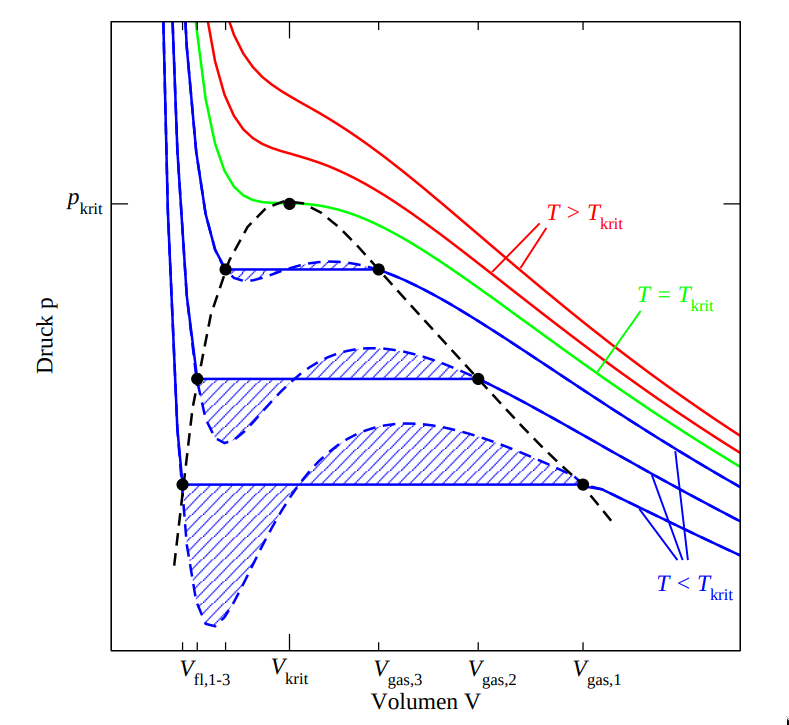
\includegraphics[width=270pt, center]{vaniso.png}
\caption{Van-der-Waals Isotherms, taken from the instructions \cite{instructions}}
\label{fig:length_eight_mouse}
\end{figure} According to Equation 3, the curves at low temperatures have two extremes and an inflection point.
In reality, however, the pressure in the area around the extrema remains constant. At the so-called critical point, the maximum, minimum and turning point coincide. The measurements at this point are called critical pressure $p_{crit}$, critical volume $V_{crit}$ and critical temperature $T_{crit}$. Here both the first and second derivatives of pressure with respect to volume are equal to zero:
\begin{equation}
    \bigg(\frac{\delta p}{\delta V}\bigg)_{T_{krit},V_{krit},p_{krit}} = 0,
\end{equation}
\begin{equation}
    \bigg(\frac{\delta^2 p}{\delta V^2}\bigg)_{T_{krit},V_{krit},p_{krit}} = 0.
\end{equation}
Applying equations 7 and 8 to the Van der Waals equation 3 gives the following relationships for the critical volume and $p_{crit}$:
\begin{equation}
    V_{krit} = 3 \cdot b \cdot n
\end{equation}
\begin{equation}
    p_{krit} = \frac{a}{27 \cdot b^2}.
\end{equation}
\paragraph{Vapor pressure}
The area under the dashed function in Figure 1 is called the coexistence region, where gas and liquid both coexist. Its boundary values are called gas volume $V_g$ and liquid volume $V_{lq}$. In the coexistence region, with a temperature-dependent constant vapor pressure $p_d$, more and more gas is converted into liquid with decreasing volume. In contrast, at $T > T_{crit}$ no more liquid is produced, no matter the pressure, and the gas can be assumed to be ideal. The slope of the dashed vapor pressure curve $p_{d}(T)$ in Figure 1 depends on the so-called vaporization enthalpy $L$:
\begin{equation}
    \frac{dp_d}{dT} = \frac{L}{T \cdot (V_g - V_{lq})}.
\end{equation}
\section{Experiment}
\paragraph{Setup}
The gas under study is sulfur hexafluoride. It is filled inside a cylinder and can be compressed with mercury, that is forced into the cylinder from the bottom. The detailed experimental setup is depicted in Figure 2.
\begin{figure}[hbt!]
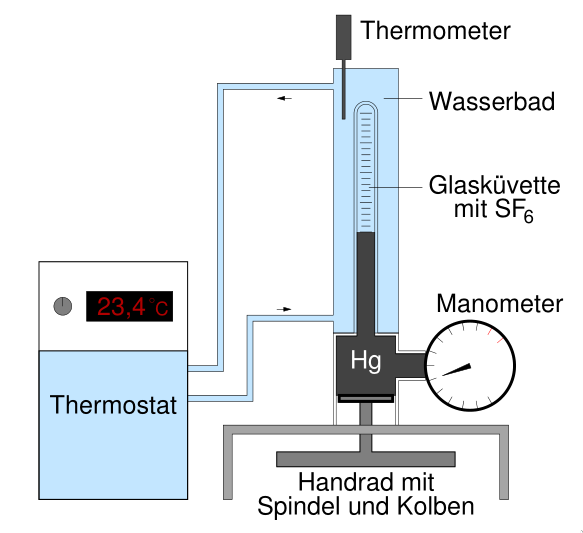
\includegraphics[width=250pt, center]{versuchsaufbau.png}
\caption{Experimental setup, taken from the instructions \cite{instructions}}
\label{fig:length_eight_mouse}
\end{figure}
The pressure put on the mercury can be read using a pressure gauge which has an estimated resolution of $25000$ Pa. The level of mercury can be read from a scale with an estimated resolution of $0.05$ cm$^3$.
\begin{figure}[hbt!]
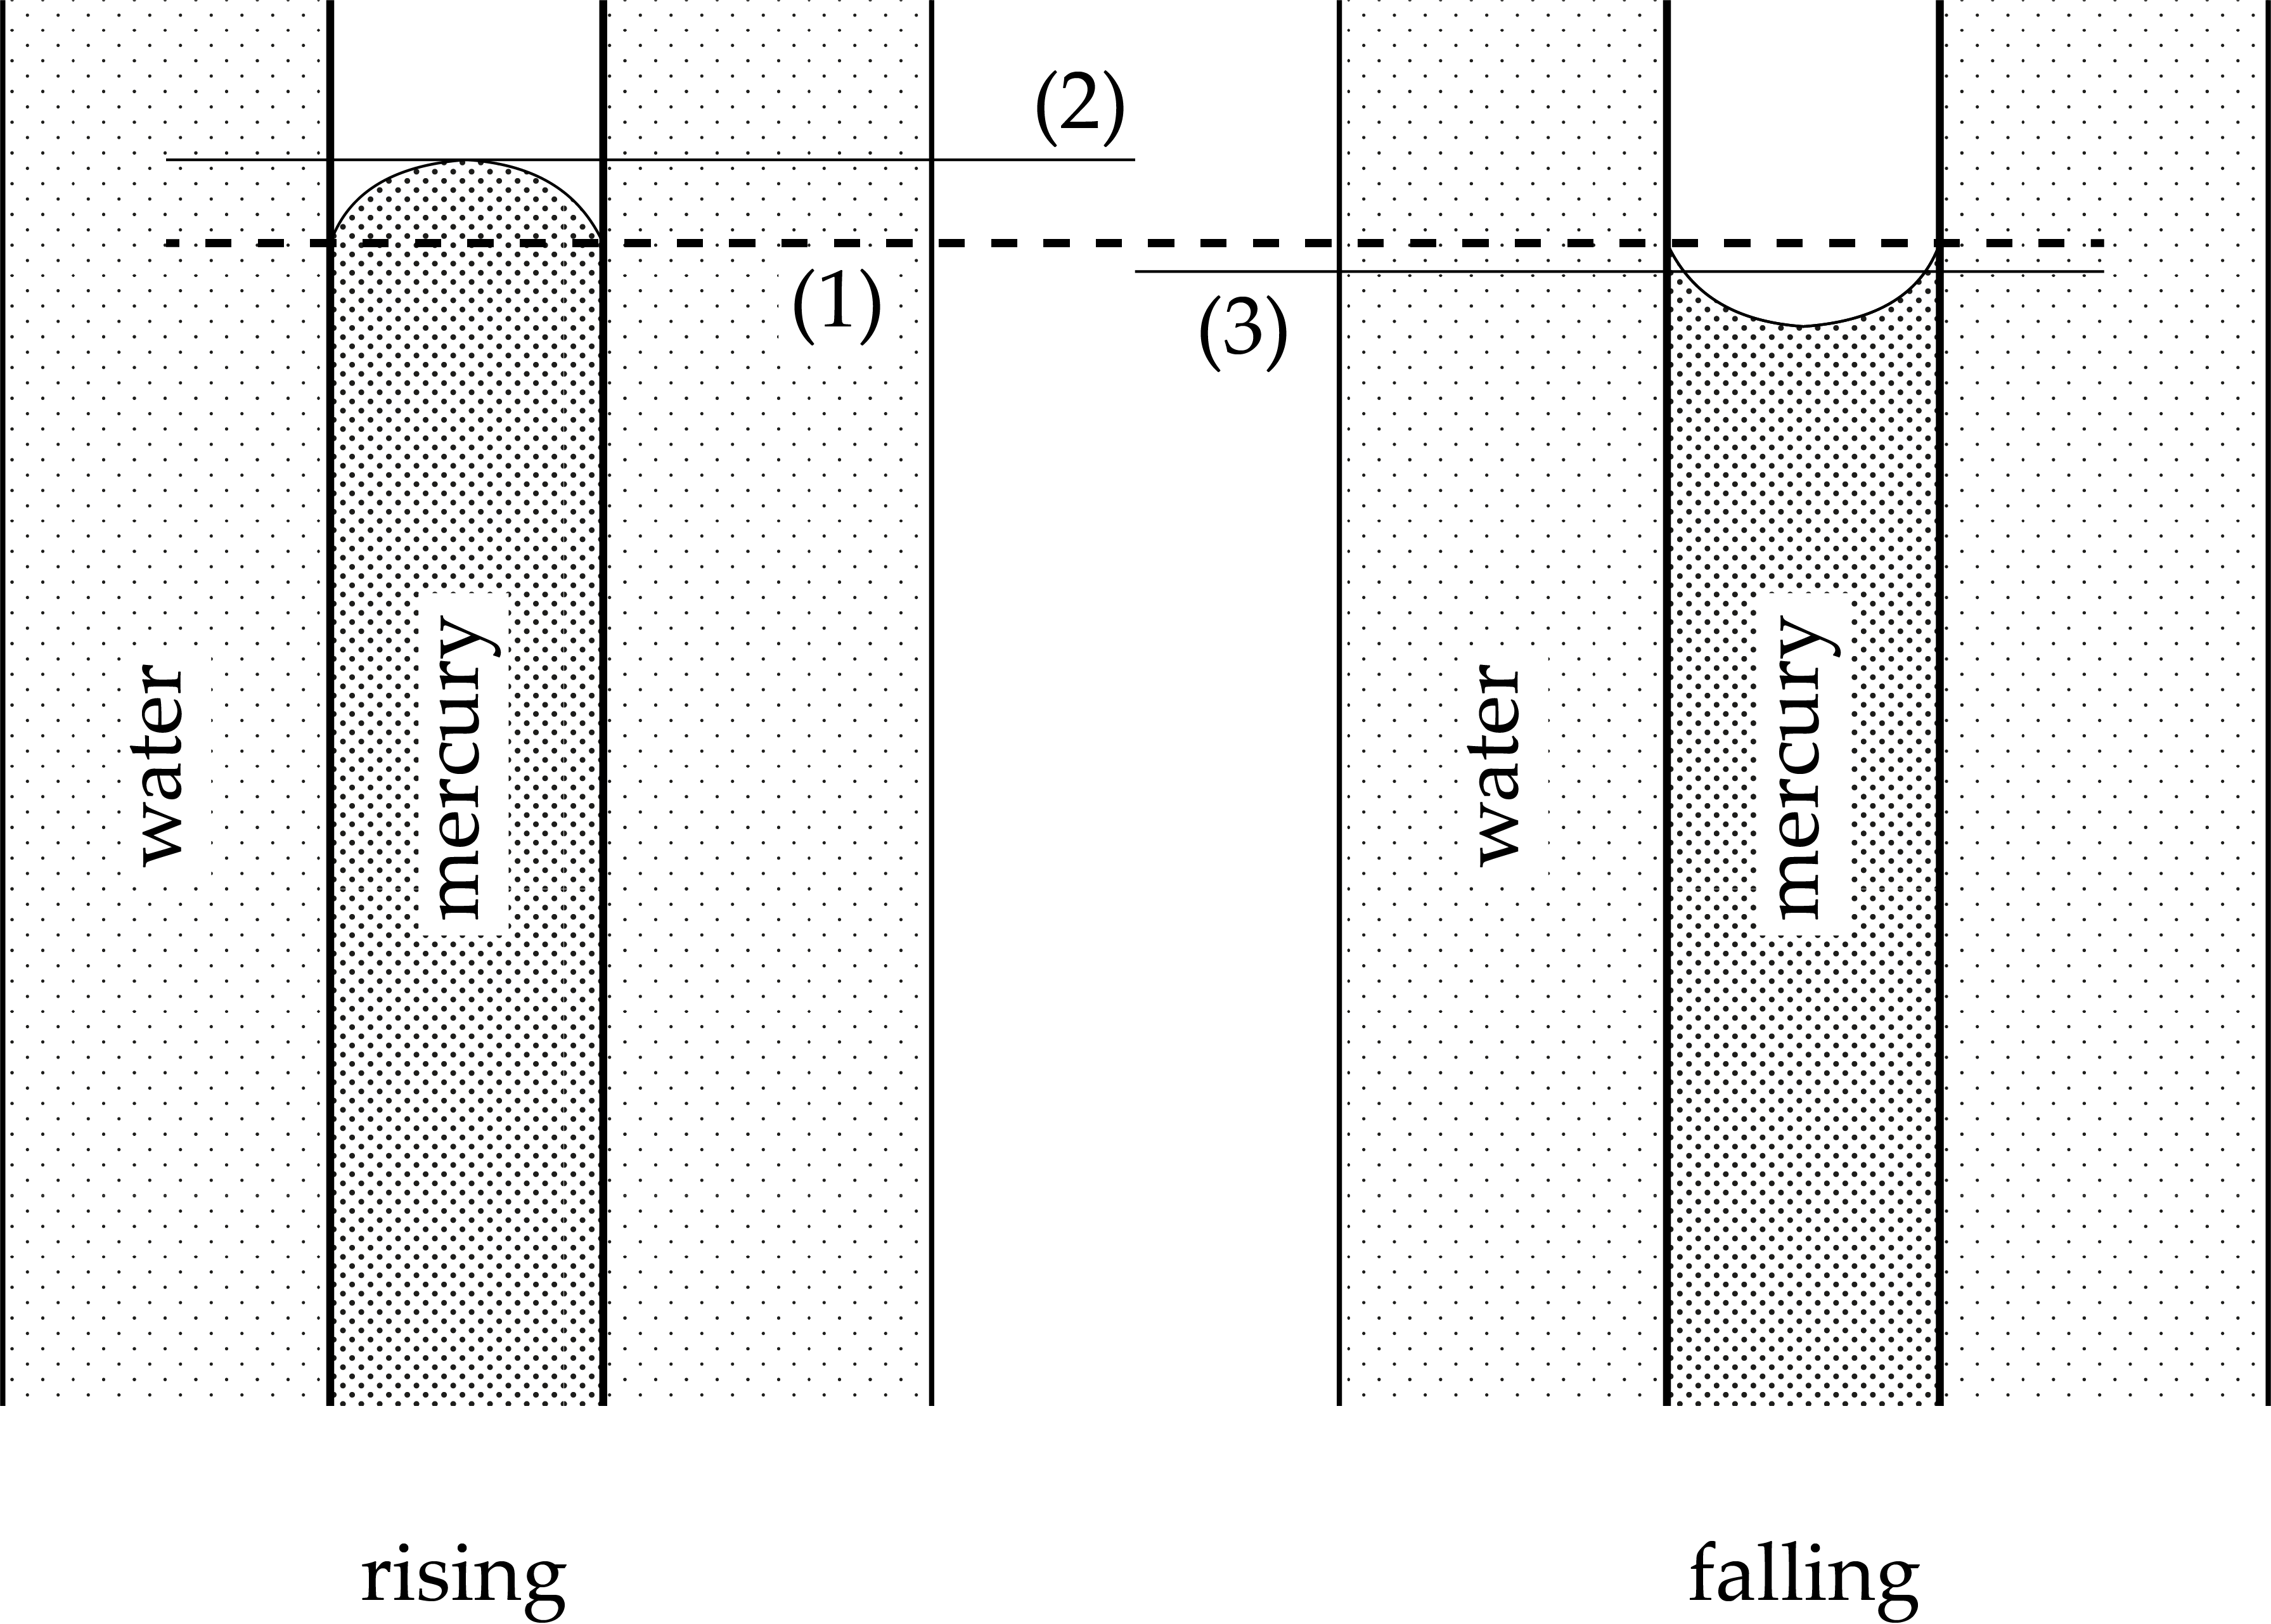
\includegraphics[width=250pt, center]{MessrohrAbweichung.png}
\caption{Error resulting from round surface}
\label{fig:length_eight_mouse}
\end{figure}
As shown in figure 3, the surface of the mercury is not flat. With both rising and falling level, a dome shaped surface forms. Because of this, the level can not be measured directly at the upper edge (1) of the mercury. Instead it is measured at roughly $\frac{1}{3}$ the distance (3) between the upper edge touching the cylinder (1) and the top of the dome (2) since 
\begin{align}
\frac{1}{4}V_{sphere}(r) = V_{Cylinder}(r,h) \cdot h\\
\frac{1}{3} r^3 = h^2 \cdot h\\
h = \frac{1}{3}r
\end{align}
This error is only taken into account during the experiment. It is not discussed any further during calculation.\\
As implied in figure 1, the cylinder filled with gas and mercury is surrounded by a cylinder filled with water. The water, and thereby the gas and mercury can be tempered using a thermostat with an accuracy of 0.1°C.

\paragraph{Measurement}

The same experiment is performed for different temperatures. Our group measured values for 30°C, 40°C and 52,5°C.
First, the water is brought to the target temperature. Next, the volume is decreased in $0.25$ cm$^3$ steps. After each reduction, and especially with low volume, the pressure needs a few seconds to settle at a value. When decreasing the volume, the pressure is initially higher than the final value and vice versa with increasing volume. The decrease of volume is stopped before the pressure reaches the maximum pressure of the gauge at $5\cdot10^6$ Pa. After reaching maximum pressure, the volume is increased in $0.25$ cm$^3$ steps. This produces two values for the pressure at a certain volume and temperature. All further calculations use the arithmetic mean of the two measured pressures whenever pressure is needed for some calculation.


\section{Measurements for determining amount of substance}

Using the same setup as described before, we perform some measurements in order to determine the amount of substance later on. With some data from the data sheet \cite{messerDataSheet} of sulfur hexafluoride, we can estimate, what temperature we need to choose in order to measure within a reasonably linear relation between pressure and volume. In this case, the temperature 52,5°C was chosen since we already performed a measurement at this temperature and it is above the critical point. In order to receive good data, the measurements for this task are performed at big volumes with small changes of volume (0,1 ml) between each measurement.\\
No separate measurement was performed. Instead, the measurements at 52,5°C from the previous task were performed with smaller changes in said interval.

\section{Calculating amount of substance}
\medskip

\paragraph{Principle}

In order to determine the molar amount of gas inside the test tube, we assume an ideal gas for further evaluation. With lower density of the gas, this approximation is more accurate.
As previously stated, an ideal gas is described by
\begin{align}
N = \cfrac{p \cdot V}{k_B \cdot T},
\end{align}
\raggedright where N describes the number of particles. Since we can only experiment with a finite volume, we extrapolate values for $p \cdot V$ by letting $V \rightarrow \infty$, thus calculating with an infinitely low density. We can determine an approximation for $p \cdot V$ by plotting $\frac{1}{V}$ against $p \cdot V$ and extrapolating the curve to $\frac{1}{V} = 0$. 

\paragraph{Error Propagation}

The value of $p \cdot V$ cannot be measured directly. Its uncertainty must be calculated by combining the uncertainties of measured values into a total uncertainty 

\begin{align}
u(p, V)  = \sqrt{\frac{\delta (p \cdot V)}{\delta p} ^2 \cdot (\Delta p)^2 + \frac{\delta (p \cdot V)}{\delta V} ^2 \cdot (\Delta V)^2} = \sqrt{V^2 \cdot (\Delta p)^2 + p^2 \cdot (\Delta V)^2}
\end{align}

where $\Delta p$ and $\Delta V$ are the uncertainties needed to be combined and $u(p,V)$ is the resulting uncertainty. Note that the uncertainty now also depends on the values $p$ and $V$ of the measurement.

\medskip

The uncertainty of the inverse volume must also be determined. In general, uncertainty for a function of the form $f(x)$ at a distance of $\Delta x$ from x is given by

\begin{align}
|\Delta f| = |\frac{df}{dx}| \cdot |\Delta x|
\end{align}

For $f(x) = x^{-1}$, this results in

\begin{align}
|\frac{d}{dx} x^{-1}| \cdot |x| = |\frac{1}{x}|
\end{align}

Thereby, the ratio of uncertainty is the same for $V$ and $V^{-1}$.

\begin{align}
u_r(\frac{1}{V}) = u_r(V) = \frac{V + \Delta V}{V} - 1 = \frac{\Delta V}{V}
\end{align}

For the uncertainty of the measurement value follows

\begin{align}
u(\frac{1}{V}) = u_r(\frac{1}{V}) \cdot V^{-1} = \frac{\Delta V}{V^2} 
\end{align}

\paragraph{Extrapolation}

\begin{figure}[hbt!]
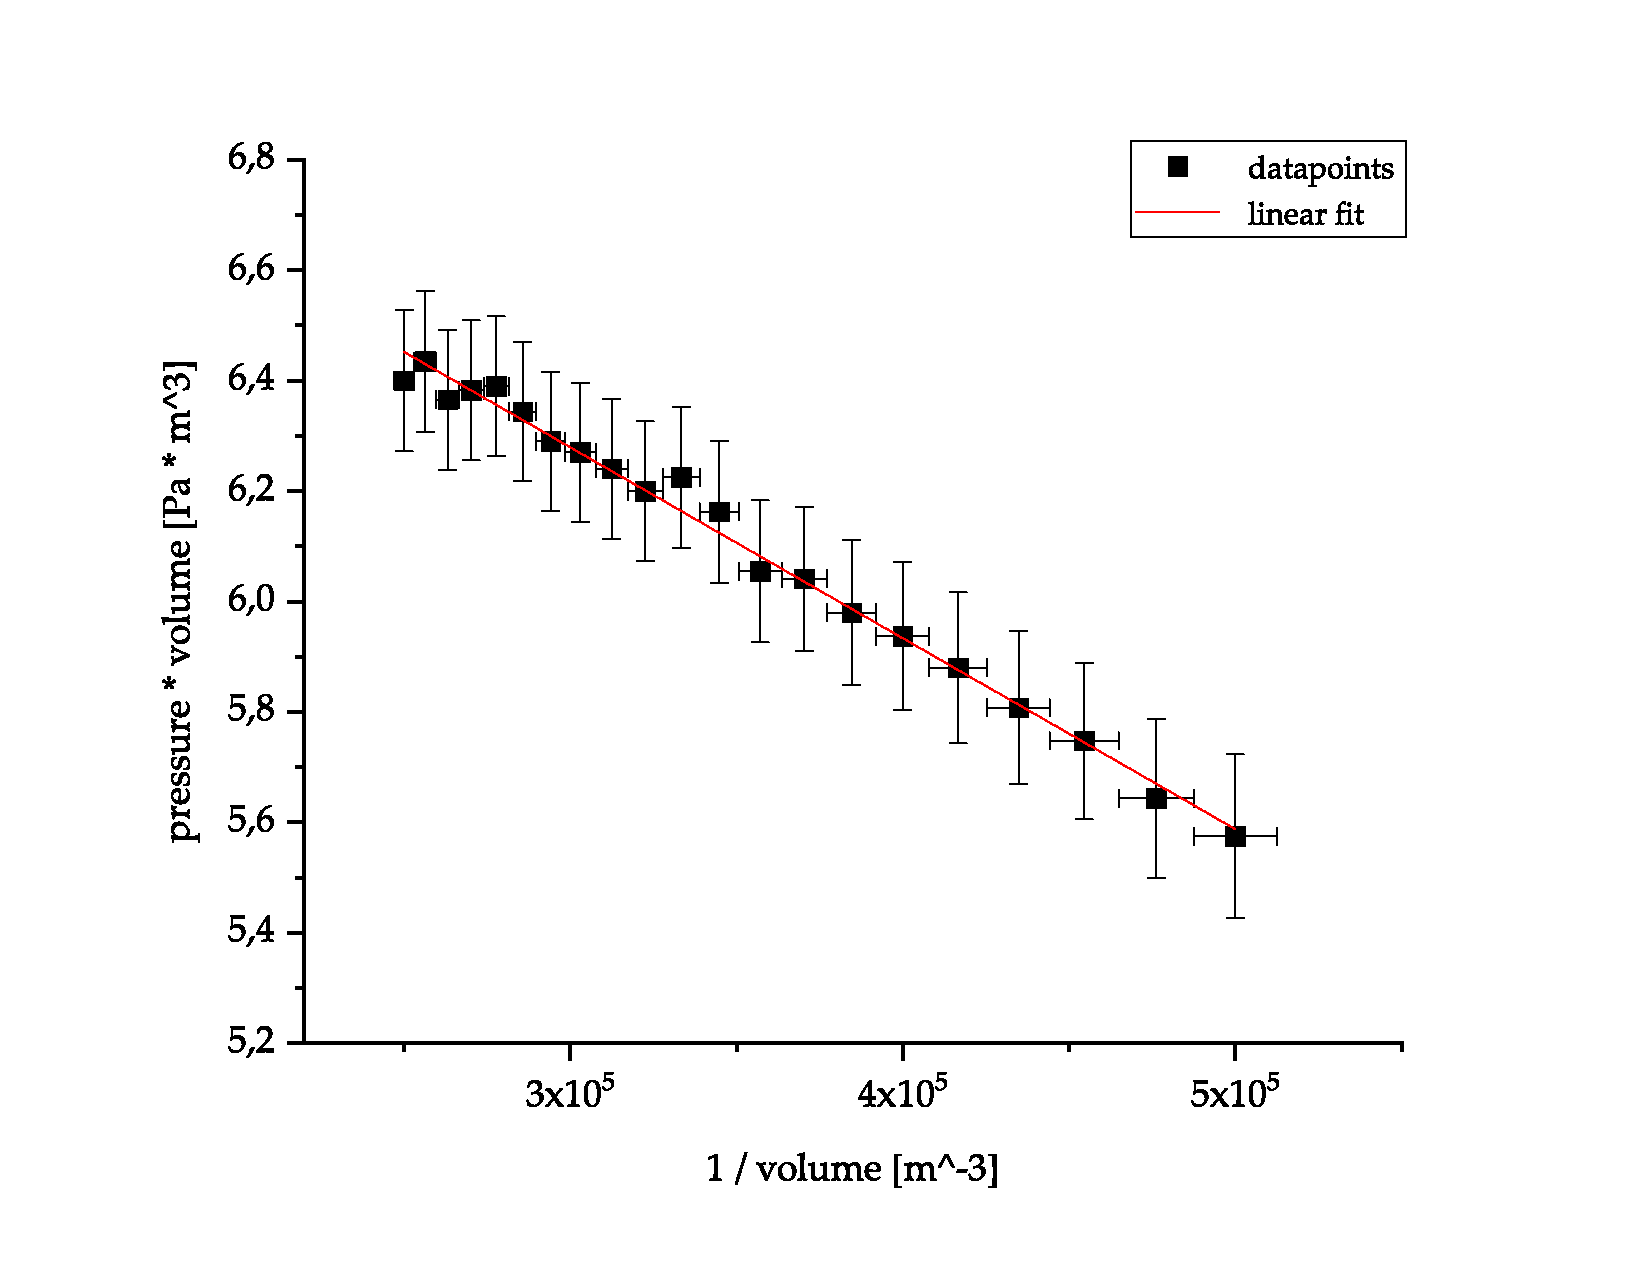
\includegraphics[width=\textwidth]{Graph2.eps}
\caption{Linear fit for extrapolation of volume $\rightarrow \infty$}
\label{fig:length_eight_mouse}
\end{figure}

In this case, the values for $\frac{1}{V}$ are represented by the x-axis. Performing a linear fit, for $x \rightarrow 0$ we receive $y \rightarrow 7.316 (0.028)$ $[\textrm{Pa} \cdot \textrm{m}^3]$

\bigskip

Using the relation
\begin{align}
n = \frac{N}{N_A}
\end{align}

with $n$ being the the molar amount and $N_A = 6.02214076 \cdot 10^{23} \cdot \frac{1}{\textrm{mol}} $ being the Avogadro-constant, we obtain
\begin{align}
n \approx 2.702 (0.010) \ \textrm{mmol}
\end{align}
for the combined temperature range.

\section{Isotherms}
\medskip

\paragraph{Molar Volume}

In order to compare measurements from different set-ups, the molar volume is useful since measurements with different amounts of gas can be directly compared.
The molar volume can be calculated from the amount of substance $n$ and the volume $V$ at a certain pressure $p$.
\begin{align}
V_m(p) = \frac{V(p)}{n}
\end{align}

\paragraph{Error Propagation}

The already known errors for $V$ and $n$ are combined using the known formula from equation (2).

\begin{align}
u(V, n) = \sqrt{(\frac{1}{n})^2\cdot (\Delta V)^2 + (\frac{V}{n^2})^2 \cdot (\Delta n)^2 }
\end{align}

The resulting values and errors fit the expected curves. Unfortunately, there is no recorded data available for when liquid starts forming unless for the dataset of 40°C. This is partly due to lack of documentation and partly due to missing data from other groups.

\paragraph{Graph}

The data in Figure 4 roughly looks as expected. At closer inspection, one can see that some of the lines cross each other, which is unexpected. Higher temperature should always result in a higher positioned line. This anomaly is probably due to calculation or measurement error. 

\section{State of aggregation}

As stated, no sufficient data about when the probe became a liquid was collected or handed out by the other groups. It can only be estimated by analyzing the slope of the lines. For figure 3, the points where the graph changes slope drastically, are used to define the transition of state of aggregation.

\begin{figure}[hbt!]
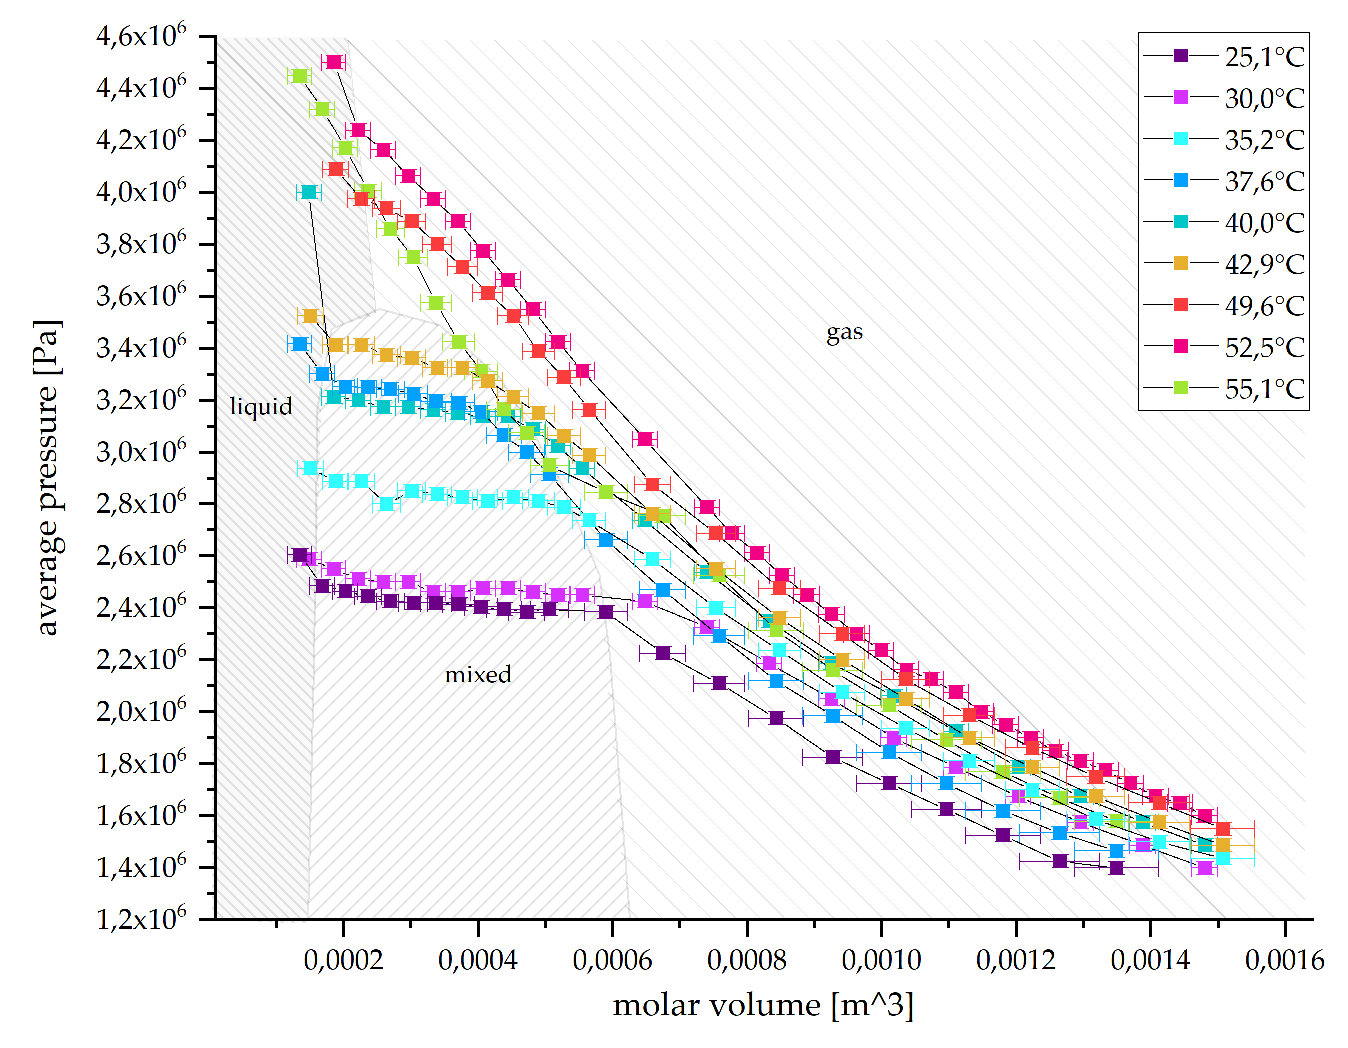
\includegraphics[width=400pt, center]{isobaresArea.eps}
\caption{State of aggregation at different pressures and temperatures}
\label{fig:length_eight_mouse}
\end{figure}


\section{Van der Waals equation}


Figure 5 shows the isotherms for sulfur hexafluoride SF6 with the limit curve for the coexistence region. We can observe that $T_{crit}$ for SF6 is somewhere between 43°C and 50°C. In fact, the literature value for $T_{crit}$ is 45.55°C.\cite{messerDataSheet}
We then approximated a limit curve for the mixed region and found a maximal, giving us the critical molar volume $V_{m,crit} = 0,25(0,05)$ l/mol and critical pressure $p_{crit} = 3,55(0,05)$ MPa.
With the critical values we can now calculate the co-volume \textbf {b} and variable \textbf{a} of the internal pressure for a single particle and 1 mol. By rearranging the following two formulas from earlier:
\begin{align*}
 V_{krit} = 3 \cdot b \cdot n \\
 p_{krit} = \frac{a}{27 \cdot b^2}
\end{align*}
and remembering that $V_{krit}$ is a molar volume we get the results in table 1.
\begin{table}[!ht]
\centering
\begin{tabular}{|l|l|l|}
\hline
 $a \ [\textrm{Pa} \cdot  \textrm{l}^2 ]$ & $(6,13 \pm 0,09) \cdot 10^{5}$  & $(1,79 \pm 0,12) \cdot 10^{-47}$ \\
 \hline
 $b \ [\textrm{l} ] $ &$ 0,08 \pm 0,02 $ & $(1,38 \pm 0,28) \cdot 10^{-25}$  \\ 
 \hline
\end{tabular}
\caption{Results for variable a and co-volume b.}
\end{table}
\section{Vapor pressure}
In order to calculate the vapor pressure from the measured isotherms, the mean value of all pressures that lie in between the coexistence region of gas and liquid shown in Figure 5 is calculated for each temperature. \\
If you now plot the vapor pressure $p_d(T)$ on a logarithmic scale against the reciprocal of the temperature $1/T$ and fit an exponential function, you get Figure 6.

\begin{figure}[hbt!]
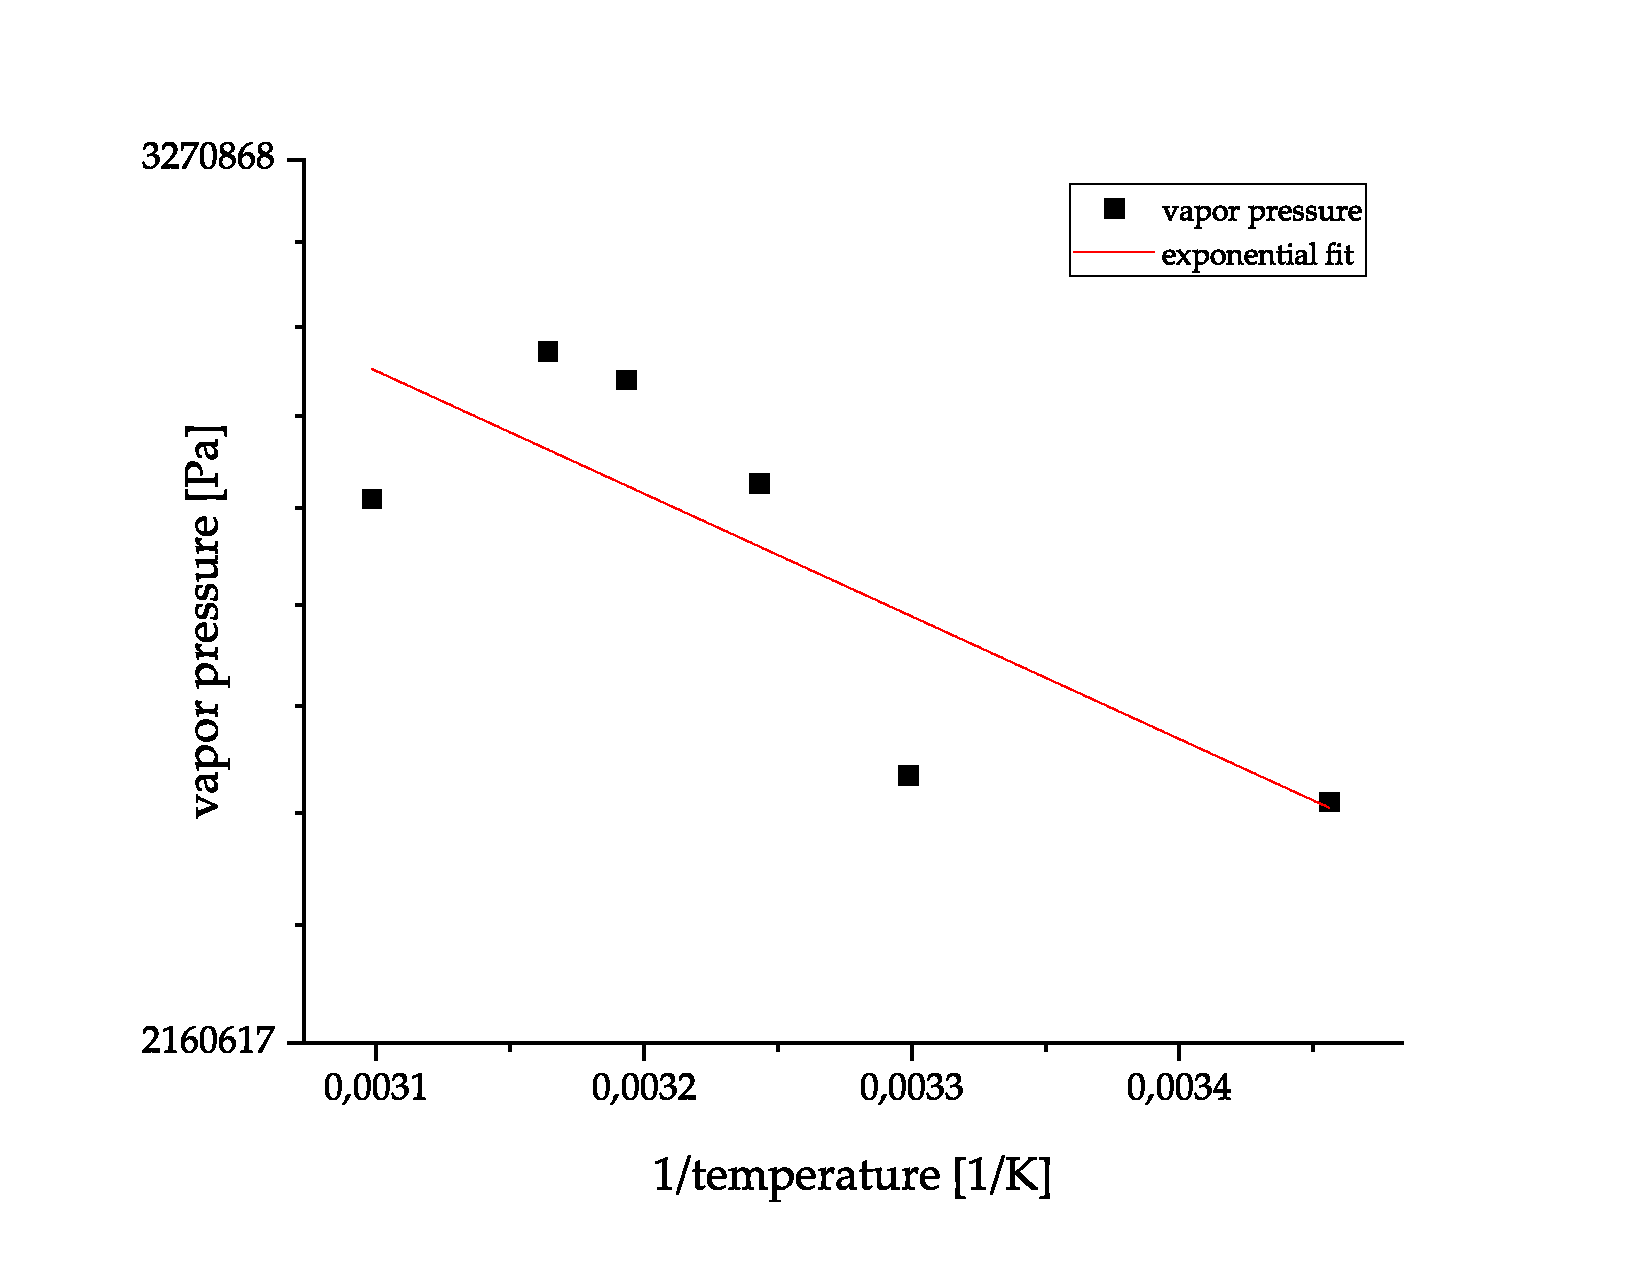
\includegraphics[width=400pt, center]{exponentialFit.eps}
\caption{Vapor pressure against the reciprocal of temperature}
\label{fig:length_eight_mouse}
\end{figure}

The semi logarithmically fitted exponential function is of the form

\begin{align}
p_d(T) = e^{k -A \cdot \cfrac{1}{T}}
\end{align}

which, plotted semi-logarithmically results in
\begin{equation}
A = -\frac{dp_d}{d\frac{1}{T}}
\end{equation}

with $A = 1865(8)$K. Inserting this value into equation 27, derived from formula 9 of the instructions \cite{instructions}, we obtain the values in table 2.

\begin{equation}
L = \frac{A \cdot p_d \cdot (V_g - V_{fl})}{T}
\end{equation}

\begin{table}[]
\centering
\begin{tabular}{|l|l|l|l|l|}
\hline
$T$[K] & $p_d$[MPa] & $V_g-V_{fl}$[$dm^3$] & $L$[$\frac{kJ}{mol}$] & $u(L)$[$\frac{kJ}{mol}$]  \\ 
\hline 
298,35 & 2,41 & 0,431 & 6,48 & 0,13\\ 
\hline 
303,15 & 2,49 & 0,426 & 6,53 & 0,13\\ 
\hline 
308,35 & 2,84 & 0,380 & 6,53 & 0,14\\ 
\hline 
312,85 & 3,17 & 0,357 & 6,75 & 0,16\\ 
\hline 
310,75 & 3,21 & 0,311 & 5,99 & 0,16\\ 
\hline 
316,05 & 3,36 & 0,268 & 5,31 & 0,16\\ 
\hline 
\end{tabular}
\caption{Results for data related to vapor pressure}
\end{table}
The uncertainty $u(L)$ is calculated using
\begin{equation}
u(L) = \sqrt{\frac{p_d \cdot \Delta V}{T}^2 \cdot u(A)^2 + \frac{A \cdot \Delta V}{T}^2 \cdot u(p_d)^2 + \frac{A \cdot p_u}{T}^2  \cdot  u(\Delta V)^2 + \frac{A \cdot p_d \cdot \Delta V}{T^2}^2  \cdot  u(T)^2}
\end{equation}

Looking at Figure 7, one observes that enthalpy becomes lower with higher temperature.

\begin{figure}[hbt!]
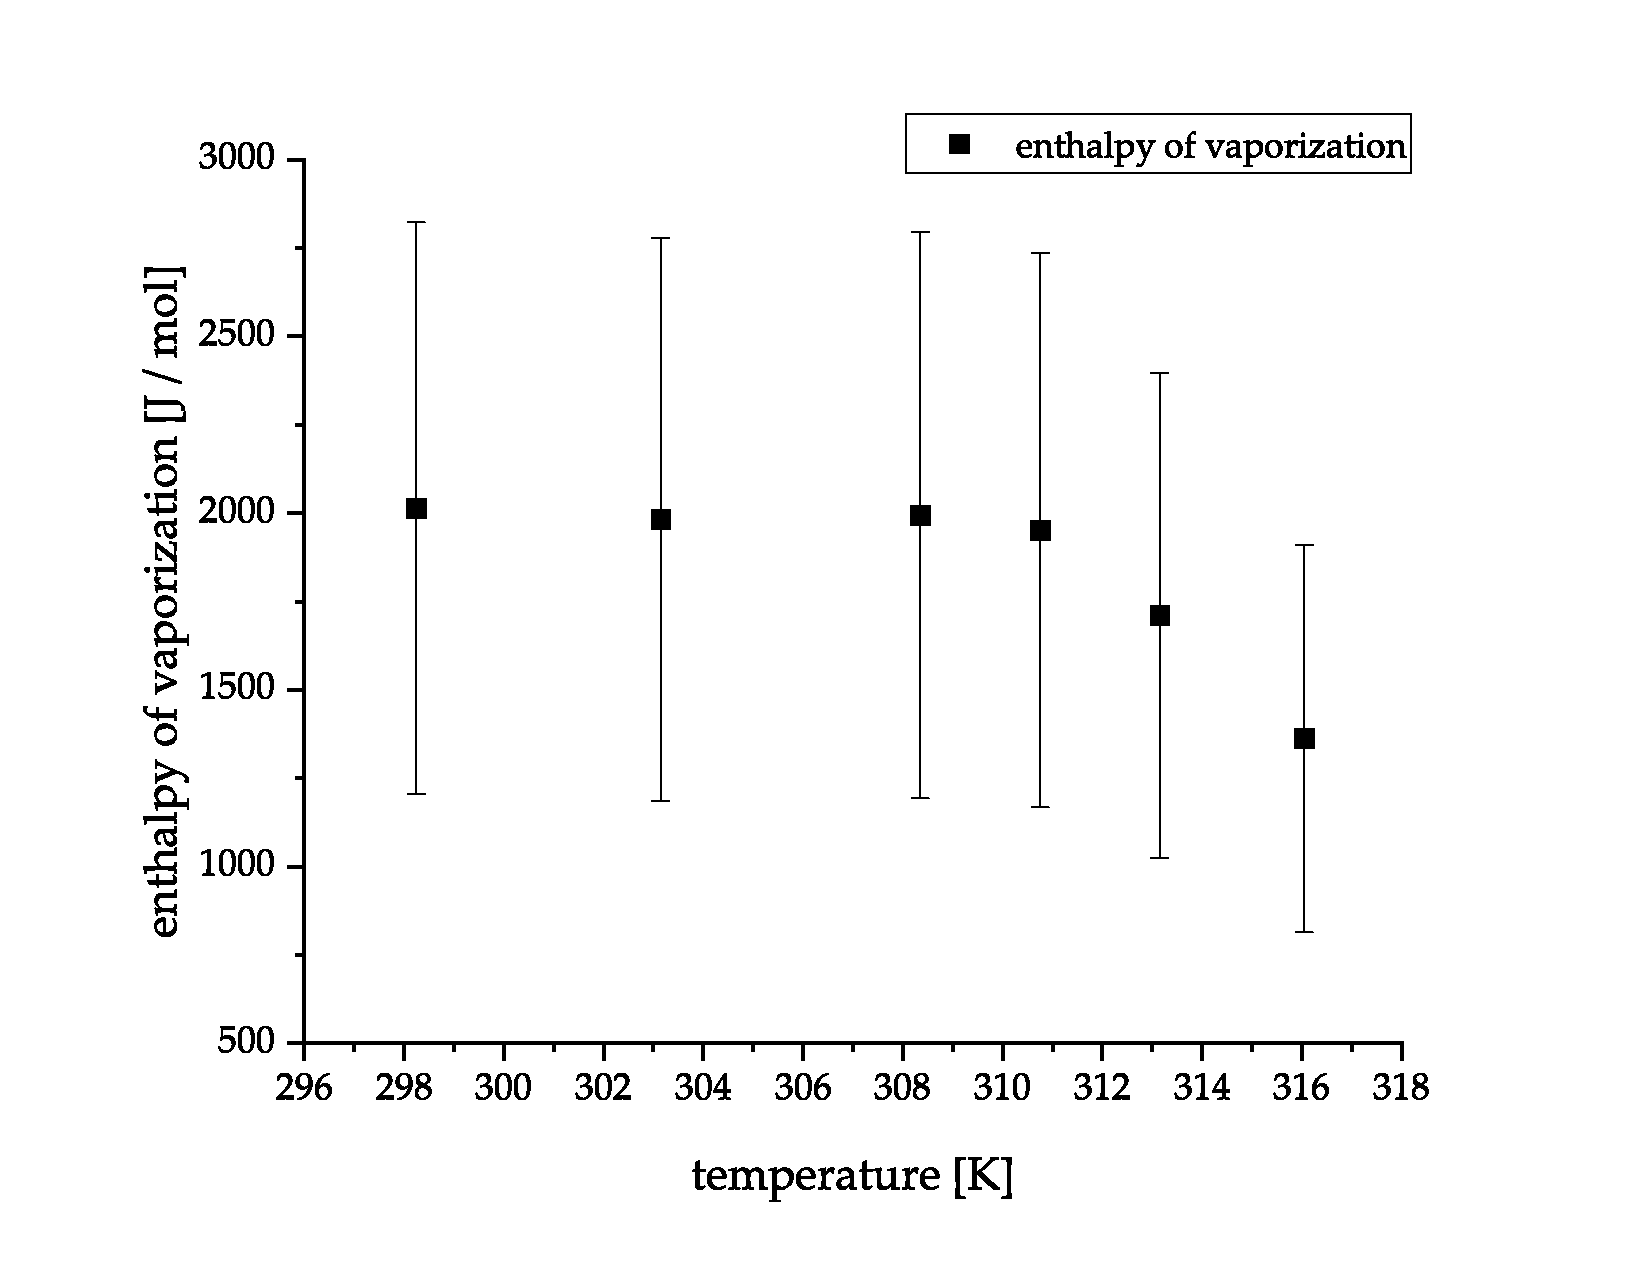
\includegraphics[width=400pt, center]{enthalpy-vs-temperature.eps}
\caption{Enthalpy of vaporization at different temperatures}
\label{fig:length_eight_mouse}
\end{figure}

\section{Comparison with literature}
\begin{table}[]
\centering
\begin{tabular}{|l|l|l|}
\hline
$V_{krit}$ & $0,198$ l/mol \cite{data} & $0,25(5)$ l/mol \\ 
\hline 
$p_{krit}$ & $3,7590 \cdot 10^6  \textrm{ Pa}$  & $3,55(5) \cdot 10^6 \textrm{Pa}$ \\ 
\hline 
a & 7,857 $\cdot 10^5  \textrm{ Pa} \cdot \ \textrm{l}^2 / \textrm{mol}^2$ \cite{handbook} & 6,13(9) $\cdot 10^5 \textrm{ Pa} \cdot \ \textrm{l}^2 / \textrm{mol}^2$ \\ 
\hline 
b & 0,0879 l/mol \cite{handbook} & 0,08(2) l/mol \\ 
\hline 
L & $ 22,37$ kJ/mol \cite{handbook} & see above \\ 
 \hline
\end{tabular}
\caption{Literature values in comparison to experimental values}
\end{table}
Taking into account the uncertainty, the critical volume is slightly above the literature value. Since the measurement quality of all groups effect this value, an error is hard to spot. During the measurements hardly any notes were taken about the aggregation state of the substance. This lead us to guess it based on the graphs. Obviously, this renders the according calculations inaccurate. These inaccuracies propagate through the values a and b. Nevertheless, Figure 7 looks as expected: with higher temperature, the enthalpy of vaporization becomes lower. The datapoint of the measurements for 312,85K $\widehat{=}$ 39,7°C is clearly influenced by some error. This starts at figure 5, where the measurements for 37,6°C lie above the values for 39,7°C, which is unexprected since the pressure for coexisting state of aggregation should rise with temperature. An error during measurement is likely.



\section{Fluctuation of pressure}

After every change of volume, pressure fluctuations continued to occur for a short time. Therefore we waited a few seconds after each change before reading the final pressure on the manometer.
The reason for this anomaly is that the gas is no longer in thermal equilibrium after the pressure change.
The increase in volume not only increases the pressure but also the temperature of the gas.
It then takes a short time for the gas to be cooled down or heated up again by the water, which is kept at the target temperature by the thermostat. \\
When changing temperature at constant volume, the pressure also changes.

\section{Attachments}
Protocol


\begin{thebibliography}{9}

  \bibitem{messerDataSheet}
  Messer Schweiz AG, Datenblatt Schwefelhexafluorid
  \textbf{URL:} \url{https://www.messer.ch/documents/2227840/4121563/Schwefelhexafluorid.pdf/47b9120b-e052-966e-3b35-527e7df3ed04?t=1595841860760}
  
  \bibitem{handbook}
  Ph.D. W.M. Haynes,
  \textit{Handbook of Chemistry and Physics},
  CRC Press.,
  ISBN: 978-1-4822-0868-9.
  
\bibitem{data}
  U.S. Secretary of Commerce, NIST Chemistry WebBook, Sulfur hexafluoride datasheet
  \textbf{URL:} \url{https://webbook.nist.gov/cgi/cbook.cgi?ID=C2551624&Mask=4}  
  
  
  \bibitem{instructions}
  Fakultät für Physik. \emph{Zustandsgleichung realer Gase} (ZUS. Technische Universität München. 10.05.2022)
  \textbf{URL:} \url{https://www.ph.tum.de/academics/org/labs/ap/ap1/ZUS.pdf}
  
  
\newpage
  
\end{thebibliography}

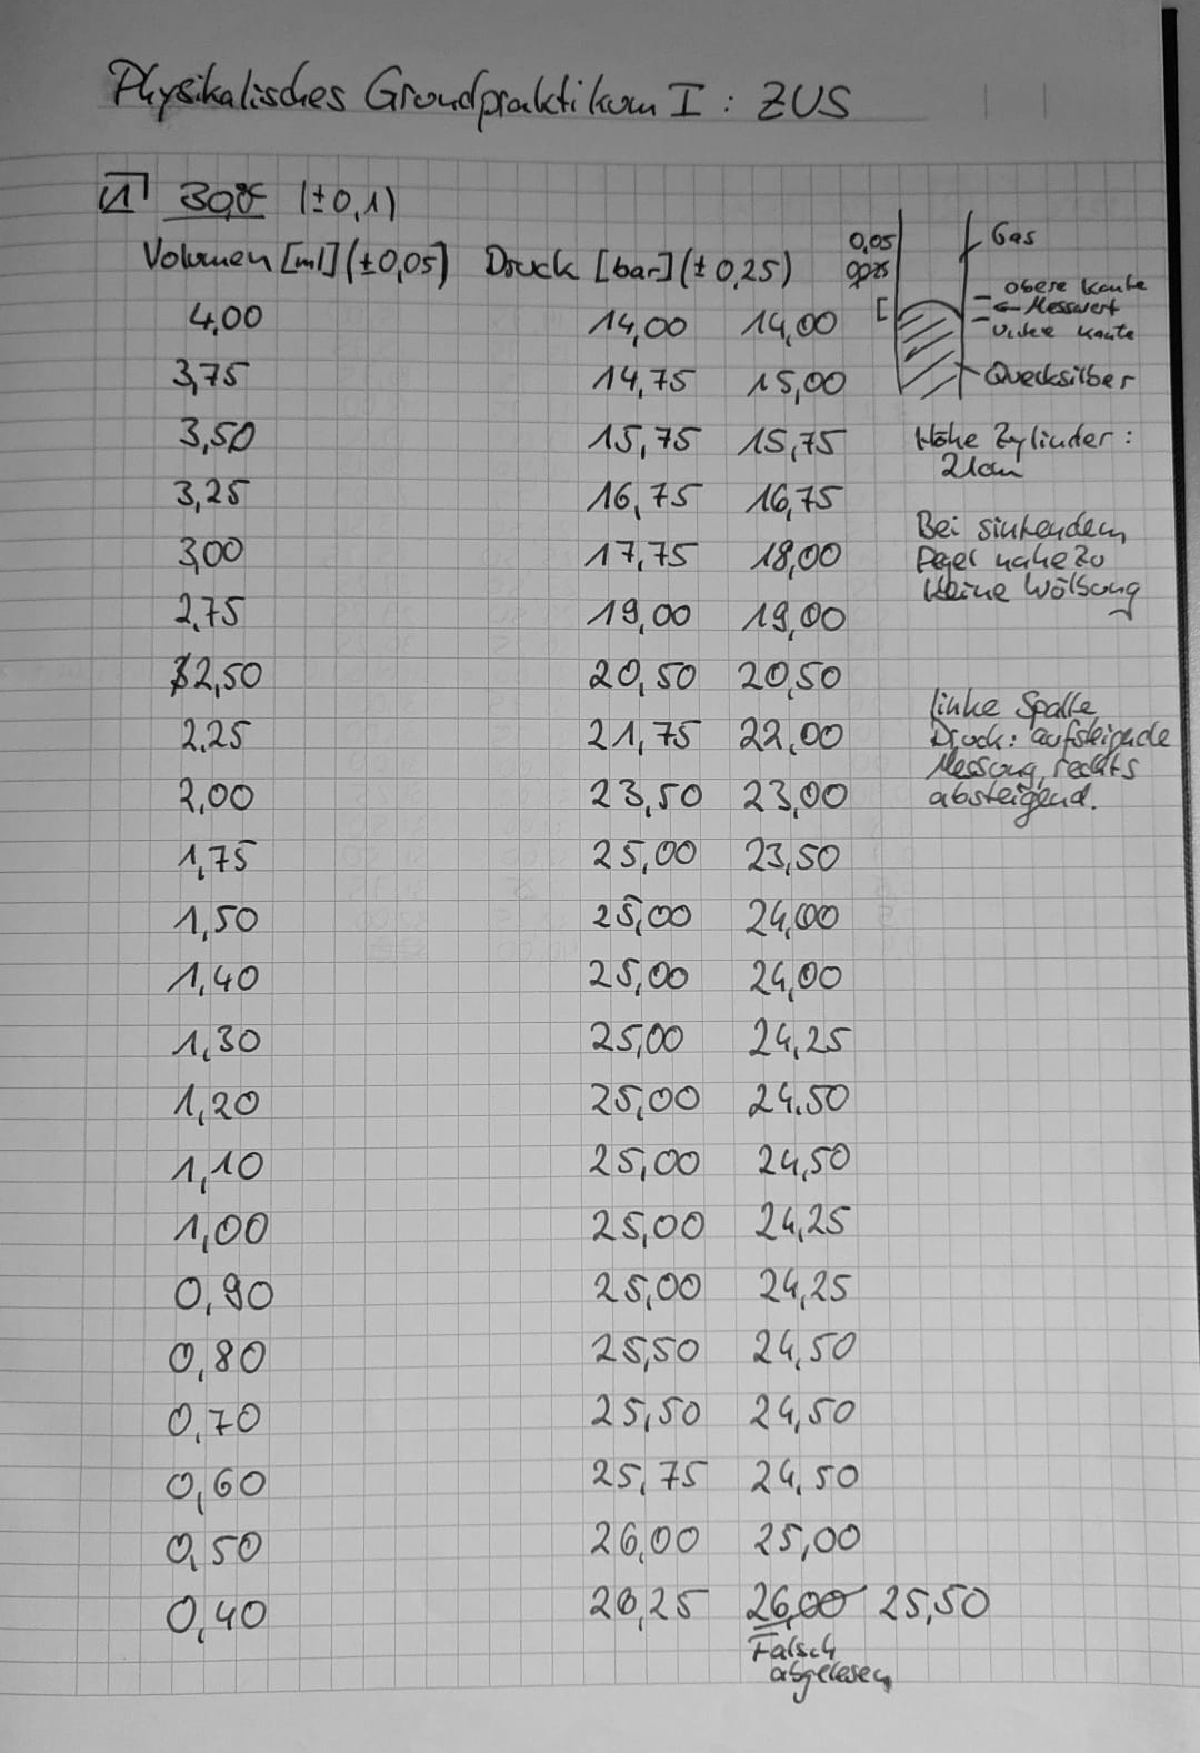
\includepdf[pages=-]{Protokoll.pdf}

\end{document}

